% change according to folder and file names
\ifpdf
    \graphicspath{{3/figures/PNG/}{3/figures/PDF/}{3/figures/}}
\else
    \graphicspath{{3/figures/EPS/}{3/figures/}}
\fi

%: ----------------------- contents from here ------------------------
\chapter{Variable correlation in Engineering problems} % top level followed by section, subsection
In any optimization problem solved with traditional EAs the exploitation of relationships between the decision variables, with respect to the objective functions, can lead to significantly faster exploration of the design space \cite{Salomon,Roy_2002a,Ghisu_2010}. 


Such relations are in the form of: if variable $a$ moves in direction $A$ then variable $b$ should move in direction $B$ with respect to any of the objectives. This type of relations between decision variables can be exploited by the EA via a simple rotation of the design space ($cite$), if known in advance. 

Unfortunately in the majority of industrial engineering cases, such as the design optimizations of hydraulic machinery, this relationships are not known in advance since they are both problem and parametrization specific. This fact along-side to many objectives, hard constraints and, usually, fragmented design space leads to significant loss of performance if compared with typical mathematical test cases ($Cite$). A way to estimate, dynamically update and use this relations is devised by as.

\section{Welded beam demonstration case}
The presence and exploitation of relationships between decision variables will be demonstrated through a known simple case, namely the minimization of both the cost ($K$) and the deflection ($\Delta$) of a welded beam subject to a force $P$ (fig. \ref{case}). There are two design variables: the side length of the square cross section ($X_2$) and the welding length ($X_1$) (fig. \ref{case}). The design is made subject to constraints o shear stress ($\tau$), bending stress ($\sigma$) and buckling load ($P_c$).   

\figuremacroW{case}{Welded beam case - Problem definition.}{In the examined case, design variables are square cross section side-length ($X_2 = t$) and welding length ($X_1 = l$) are the design variables.}{0.4}

The problem can be formulated as,

Minimize Cost,
%\begin{equation} 
\begin{eqnarray}\nonumber
   K = 1.10471h^2l+0.04811t^2(14.0+l) \\
   = 1.10471h^2X_1+0.04811X_2^2(14.0+X_1)
   \label{Cost} 
\end{eqnarray}
and minimize Deflection,
%\end{equation}
\begin{eqnarray}
   \Delta = \frac{4PL^3}{Et^4} = \frac{4PL^3}{EX_2^4}
   \label{Deflection} 
\end{eqnarray}

Subject to:


Constraint concerning the shear stress applied on the welding in order to ensure the structural integrity of the welding. Maximum shear stress depends on the type and quality of the welding. 
\begin{eqnarray}
   \tau = \sqrt{\tau_1^2 + \frac{\tau_1 \tau_2 l}{R} +\tau_2^2} \\
   \nonumber \tau \leq 13,600 psi \\
   \nonumber where:~~~~~~~~~~~~~~~~~~~~~~.\\
   \nonumber \tau_1 = \frac{P}{\sqrt{2}hl} \\
   \nonumber \tau_2 = \frac{MR}{J} \\   
   \nonumber M = P(L+\frac{l}{2}) \\ 
   \nonumber R = \sqrt{\frac{l^2}{4} + (\frac{h+t}{2})^2} \\
   \nonumber J = 2\left( \sqrt{2}hl\left( \frac{l^2}{12} + \left(\frac{h+t}{2}\right)^2 \right) \right)
   \label{shear} 
\end{eqnarray}

concerning the bending stress applied on the beam, to ensure structural integrity of the beam. Maximum bending stress depends on the beam material.
\begin{eqnarray}
   \sigma = \frac{6PL}{t^3} \leq 30,000 psi
   \label{bend} 
\end{eqnarray}

and concerning the buckling load, to avoid buckling phenomena.  
\begin{eqnarray}
   P_c = \frac{4.013E\sqrt{\frac{t^8}{36}}}{L^2}\left( 1- \frac{t}{2L}\sqrt{\frac{E}{4G}} \right) \\
   \nonumber  P - P_c \leq 0 
   \label{back} 
\end{eqnarray}
,where welding hight is $h = 0.6 in$, beam reach is $L = 14 in$, the extend of the force is $P = 6000 lb$, Young’s modulus is $E = 30 \times 10^6 psi$, and shear modulus is $G = 12 \times 10^6 psi$.  

Apart from the structural, constraints are also enforced on the objectives to bound the Pareto front within logical values, thus:

\begin{eqnarray}
   K \leq 50 \\
   \Delta \leq 0.25 
   \label{obj} 
\end{eqnarray}


\begin{figure}[h!]
\begin{minipage}[b]{0.5\linewidth}
 \centering
 \resizebox*{7.5cm}{!}{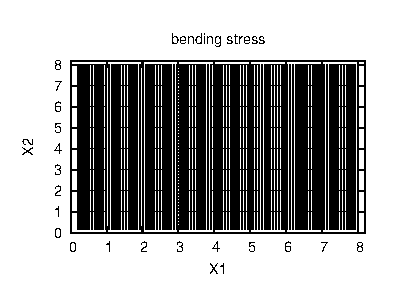
\includegraphics{Const_sx.eps}}
\end{minipage}
\begin{minipage}[b]{0.5\linewidth}
 \centering
 \resizebox*{7.5cm}{!}{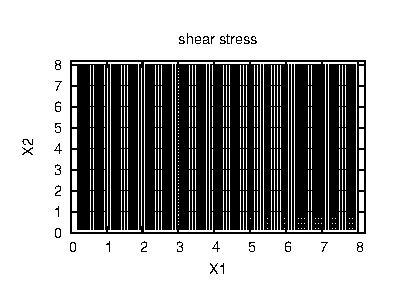
\includegraphics{Const_tx.eps}}
\end{minipage}
\begin{minipage}[b]{0.5\linewidth}
 \centering
 \resizebox*{7.5cm}{!}{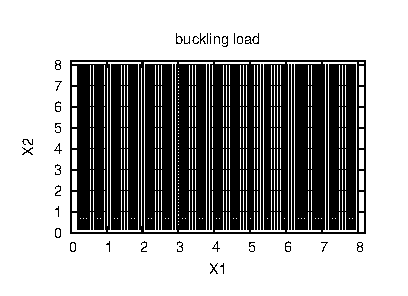
\includegraphics{Const_P.eps}}
\end{minipage}
\begin{minipage}[b]{0.5\linewidth}
 \centering
 \resizebox*{7.5cm}{!}{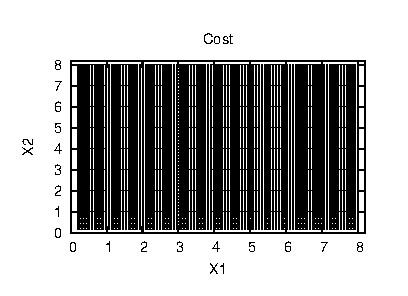
\includegraphics{Const_Price.eps}}
\end{minipage}
\begin{minipage}[b]{0.5\linewidth}
 \centering
 \resizebox*{7.5cm}{!}{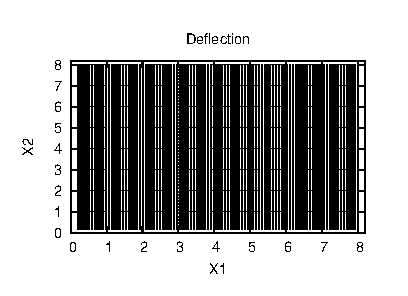
\includegraphics{Const_Dx.eps}}
\end{minipage}
\begin{minipage}[b]{0.5\linewidth}
 \centering
 \resizebox*{7.5cm}{!}{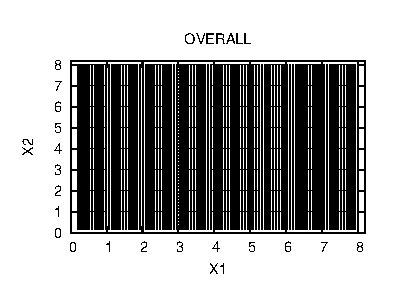
\includegraphics{Const_ALL.eps}}
\end{minipage}

\caption{Investigation of the feasibility of the design $(X_1,X_2)$ plane. The overall feasible design space is presented in the lower right figure with white squares. Constraints buckling load and maximum deflection  are both overpowered by bending stress and could be eliminated.} 
\label{x1x2}
\end{figure}


\paragraph{}
This case was deliberately chosen as a demonstration case due to the clear physical meaning of the relations that appear between its design variables. By carefully examining the objectives it is clear that in order to decrease deflection $X_1$ must be increased(eq. \ref{Deflection}). However any increase in $X_1$ will lead to higher cost (eq. \ref{Cost} ). In order to keep cost stable $X_2$ must simultaneously decrease, this of-course is bounded by the structural constraints (eq. \ref{shear},\ref{bend} and \ref{back}). 
 
This type of relations appear in all multiobjective cases. As long as a Pareto front is sought then a relation between the objectives exist $G(F_1,F_2)=0$ (fig. \ref{pareto_DOFs} -right) and since $F_i=f(X_1,X_2)$, $_i=1,2$ (eq. \ref{Cost},\ref{Deflection}) a relation between the design variables also exist $G'(X_1,X_2)=0$. The relation between the design variables can be shown if the pareto members are plotted in the design plane (fig. \ref{pareto_DOFs} -right).

\begin{figure}[h!]
\begin{minipage}[b]{0.5\linewidth}
 \centering
 \resizebox*{7.5cm}{!}{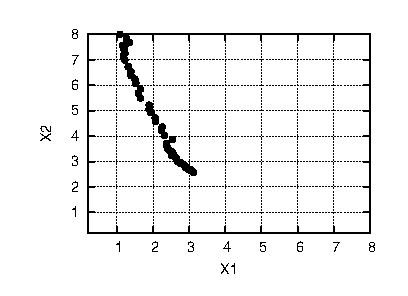
\includegraphics{DOFs.eps}}
\end{minipage}
\begin{minipage}[b]{0.5\linewidth}
 \centering
 \resizebox*{7.5cm}{!}{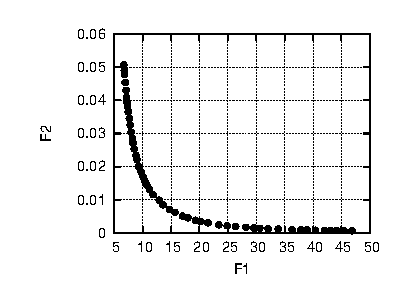
\includegraphics{Pareto.eps}}
\end{minipage}
\caption{Members of the Pareto front plotted on the design space (left) and objective space (right). For the pareto members the correlation described above is obvious.  Pareto members lay on a small band with respect to the above observations.}
\label{pareto_DOFs}
\end{figure}

EAs exploit the relationships between decision variables via rotating their design space in order to align it to the relations directions and by that influence the offspring probability distribution on the design space in order to maximise the probability of an individual to appear on the Pareto front. Regarding Crossover, since it takes place for each variable separately the probability distribution is bounded by a dof-dimentional hyber-cube (box for two objectives) aligned with the coordinate system it is applied on (fig \ref{xover}). To demonstrate how the probability distribution changes we use as an example 2 hypothetical parents plot the offspring probability distribution and based on that the probability of an individual to appear on the Pareto front(fig \ref{xover}). The probability of a individual to appear on the Pareto front is proportional to the length of the Pareto front interception line (fig \ref{xover}). For mutation, if the mutation probability is $p_m$ it is more probable to have a mutations happen on one of the axises of the coordinate system ($p_m$) and less probable as the number ($s$) of axises that have to simultaneously suffer mutation increases ($p_m^s$) (fig. \ref{mut}).      



\begin{figure}[h!]
\begin{minipage}[b]{0.5\linewidth}
 \centering
 \resizebox*{7.0cm}{!}{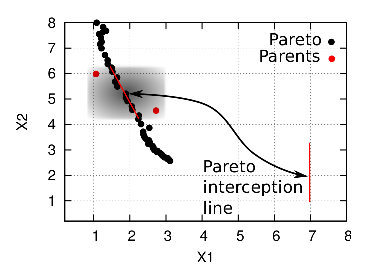
\includegraphics{DOFs_Xover2.eps}}
\end{minipage}
\begin{minipage}[b]{0.5\linewidth}
 \centering
 \resizebox*{7.0cm}{!}{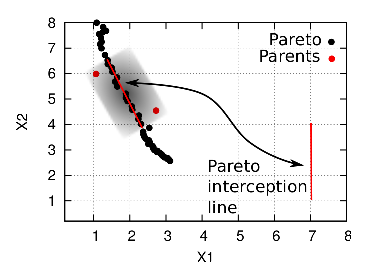
\includegraphics{DOFs_Xover.eps}}
\end{minipage}
\caption{Crossover offspring probability distribution bounding boxes as applied for original design plane (left) and the variable-relations-based rotated one (right). Pareto front interception line is significantly larger when crossover is applied on the rotated. "Extrapolation" magnitude and propability distribution in the bounding box depends on the crossover operator in use.}
\label{xover}
\end{figure}

The directions that describe the relations between design variables can be estimated at each generation via a statistical tool (principal component analysis -PCA) on current elite set and updated continuously as the elite set tents to approximate the actual pareto front. 

\begin{figure}[h!]
\begin{minipage}[b]{0.5\linewidth}
 \centering
 \resizebox*{7.0cm}{!}{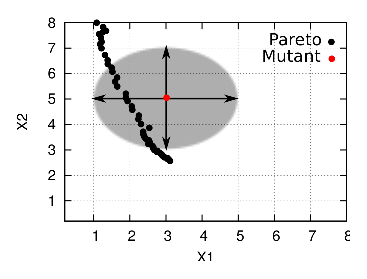
\includegraphics{DOFs_mut.eps}}
\end{minipage}
\begin{minipage}[b]{0.5\linewidth}
 \centering
 \resizebox*{7.0cm}{!}{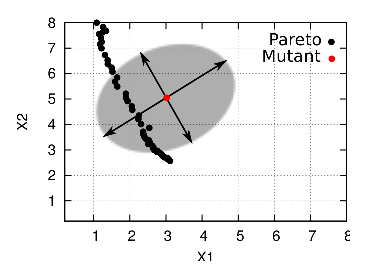
\includegraphics{DOFs_mut2.eps}}
\end{minipage}
\caption{Mutation offspring probability distribution as applied for original design variables (left) and the correlation based directions (right). Mutation in direction one is essential for improving the pareto representation quality and mutation on direction two to advance the current elite front towards the real pareto front. Both of them are equally valuable for an optimization procedure and the probability of them to happen decreases exponentially with the number of the correlated design variables.}
\label{mut}
\end{figure}

\section{Exploiting relationships between decision variables via PCA driven evolutionary operators}
PCA is an eigenvector--based multivariate analysis, performed on a data--set, that transforms possibly correlated variable sets into uncorrelated ones known as principal components. The latter are the direction vectors that best represent the variance in the data--set, \cite{Haykin,Jolliffe_2002}.

Previous implementations of the PCA technique within optimization methods, \cite{Fodor_2002, Ghisu_2010}, aimed principally at dimensionality reduction. Generally, in these works, PCA locates the directions of maximum variance in the original input data and rotates the data along these axes. Since the first principal components contain most of the necessary information, PCA can extract a small number of important components from the high-dimensional original data (which a hypersurface is to be fitted to) while retaining the important features. So, in case there is no sufficient data points to adequately populate the highly dimensional space, the metamodel may ignore the ``unnecessary'' input variables, concentrate on a lower-dimensional part of the high-dimensional space and improve, thus, a lot its prediction ability. 

Here the role of PCA is absolutely different. In specific, its role is to better ``drive'' the evolution operators by reviling the directions that describe the variable correlation.  
To be more specific, the candidate solutions are handled with all design variables, i.e. all unknowns. No (direct, at least) dimensionality reduction takes place. PCA is used to identify the most important directions in the highly dimensional design space. The design space is, then, temporarily aligned with these directions, the necessary evolution operators apply to the so--rotated individuals and, finally, the generated offspring are transformed back to the original design space. Any sort of dimensionality reduction or rotation of the design space occurs just before (and after) the application of the evolution operators. To initiate PCA, a small number of representative solutions to the problem must be available; this set is dynamically updated during the evolution. In MOO applications, this comprises the members of the current front of non--dominated solutions. In SOO problems, in which there is no set of non--dominated solutions, the principal components can be found by processing a user--defined number of top individuals in the current offspring population. It is evident that, as the evolution proceeds, and the current front of non--dominated solutions converges to the Pareto front, the principal components approach those of the Pareto front. 

By assuming the current elite set to be a standardized data--set ($X$) with the empirical covariance matrix, \cite{Fodor_2002, Jolliffe_2002},

\begin{equation} 
   P_{N\times N}= \frac{1}{e}XX^T
   \label{Cov_Mat} 
\end{equation}
where $e$ is the size of $S_e$, we can use the spectral decomposition theorem, \cite{Axler_1997, Fodor_2002}, to write $P$ as

\begin{equation} 
   P_{N\times N}= U\Lambda U^T
   \label{spectral}
\end{equation}
where $\Lambda\!=\!diag(\lambda_1 , . . . , \lambda_n )$ is the diagonal matrix with the eigenvalues of $P$ and $U$ is a $N\!\times\!N$ matrix containing the eigenvectors.

Let the aligned to the principal components design vectors \(\overrightarrow{x_i}\) be represented by \(\overrightarrow{x^*_i}\). The alignment is performed as follows
\begin{equation} 
   \overrightarrow{x^*_i}=U(\overrightarrow{x_i}-\mu_{X})
   \label{align} %http://users.ics.tkk.fi/jhollmen/dippa/node30.html
\end{equation}
where $\mu_{X}$ is the vector of mean (over the elite set) design variables.
The inverse transformation, from $x^*_i$ to $x_i$, is given by
\begin{equation} 
   \overrightarrow{x_i}=U^{-1}\overrightarrow{x^*_i}+\mu_{X}
	\label{re-align}
\end{equation}
It is important to note that the CPU cost to compute \(U^{-1}\) is negligible since U is an orthogonal matrix and, thus, \(U^{-1} = U^T\). 
\paragraph{}
%%%%%%%%%%%%%%%%%%%%%%%%%%%%%%%%%%%%%%%%%
{\bf The PCA--driven MAEA (MAEA(PCA)) fig.\ref{MAEAPCA2} :}
%%%%%%%%%%%%%%%%%%%%%%%%%%%%%%%%%%%%%%%%%

Let us denote the generation counter by $g$, the number of current entries into the DB by $k_{DB}$ and the minimum number of entries needed to initiate the use of the metamodel--based pre--evaluation phase by $k_{min}$. Then, the steps of the PCA--driven MAEA can be described as follows:
\begin{description}
  \item[Step 1:] For the current offspring population $S^{g}_\lambda$, set $\lambda^*\!=\!\lambda$ (if $k_{DB}\!<\!k_{min}$) or  $\lambda^*\!=\!\lambda_{ex}$ (else). 
  \item[Step 2:] If $k_{DB}\!\ge\!k_{min}$, train $\lambda$ RBF networks on paired input--output patterns selected from the DB, in the vicinity of each offspring. Pre--evaluate the $\lambda$ population members on the so--trained metamodels. Select the $\lambda_{ex}$ top of them, based on dominality and proximity criteria.
  \item[Step 3:] Evaluate the $\lambda_{ex}$ offspring on the problem--specific evaluation software. Update $S^{g}_e$.
  \item[Step 4:] Compute the current set of principal components based on the updated elite set $S^{g}_e$ (eqs. \ref{Cov_Mat} and \ref{spectral}).
  \item[Step 5:] Align the design space to so--computed principal components (eq. \ref{align}). 
  \item[Step 6:] Create the new offspring population $S^{g+1}_\lambda$ through the application of the evolution operator on the aligned individuals. Re--align the generated offspring to the original design space coordinate system,(eq.~\ref{re-align}).
  \item[Step 7:] Set $g\!\leftarrow\!g\!+\!1$; go to step 1.
\end{description}
The above algorithm can readily be transformed to EA(PCA) by eliminating the use of metamodels or by setting $k_{min}$ to a practically infinite number.  To transform the objecive function vectors into scalar quantities, SPEA2 (\cite{kn:Zitz02}) is used; however, this is not restrictive at all.

In order to demonstrate the possible performance gain from the use of the PCA--driven EA ten runs for the aforementioned (Welded beam) case was performed with different random number generator seeding. The average hypervolume indicator in respect to evaluations, over the ten runs, is presented in fig. \ref{HypervolumeComparison}.

\figuremacroW{HypervolumeComparison}{Hypervolume Comparison}{Hypervolume comparison between EA and EA(PCA), metamodels where not used due to the fast evaluation time of the welded beam case. EA(PCA) outperforms traditional EA even though the dimensionality of the problem in hand is very low.}{0.9}

\figuremacroW{MAEAPCA2}{MAEA-PCA}{Schematic representation of the PCA-driven MAEA algorithm.}{1.0}



% ---------------------------------------------------------------------------
% ----------------------- end of thesis sub-document ------------------------
% ---------------------------------------------------------------------------